\chapter{Vurdering af mekaniske delkoncepter til screening skema} \label{Bilag mekaniske delkonceptervurdering}

\plainbreak{-2}
\begin{figure}[H]
    \centering
     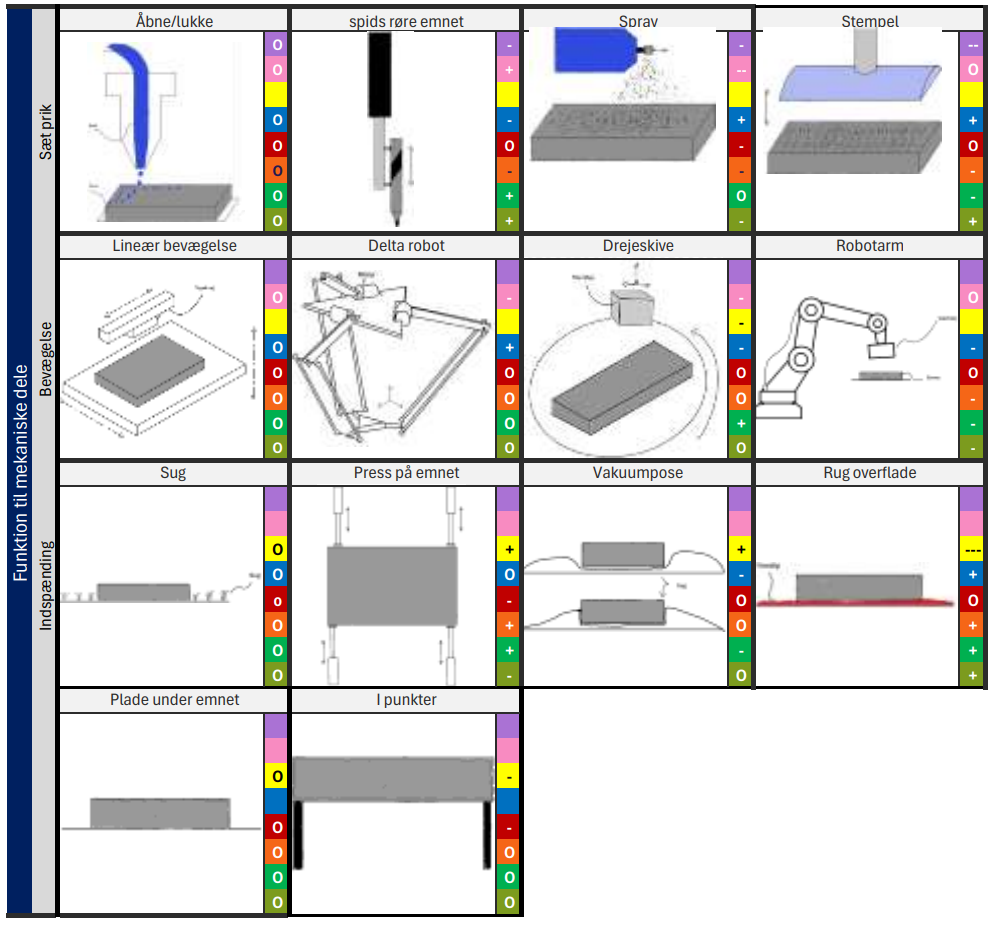
\includegraphics[width=.95\linewidth]{bilag/Media/Media/delkoncept mekanisk.png}
     \caption{Vurdering af delløsninger til mekaniske delfunktioner}
\end{figure}

\begin{table}[H]
    \centering
    \caption{Forklaring af vurderingskriterier til }
    \begin{tabular}{|l|p{9cm}|} \hline
        \rowcolor{gray!20} Vurderingskriterier & Betydning af kriteriet \\ \hline
         \multicolumn{1}{|l|}{\cellcolor{lillaB} \color{white} \textbf{Præcision af størrelse}}  & Præcision af prikstørrelse, desto lavere desto bedre\\  \hline
         \multicolumn{1}{|l|}{\cellcolor{pinkB} \color{white} \textbf{Præcision af placering}}  & Præcision af prikplacering, desto lavere desto bedre \\  \hline
         \multicolumn{1}{|l|}{\cellcolor{gulB} \textbf{Fastholdelse}}  & Egenskaben til at fastholde emnet, desto større desto bedre \\  \hline
         \multicolumn{1}{|l|}{\cellcolor{blueB} \color{white} \textbf{Hurtighed}}  & Hastigheden fra der skal laves en prøve til prøven er færdig, desto højere desto bedre \\\hline
         \multicolumn{1}{|l|}{\cellcolor{redB} \color{white} \textbf{Brugerinvolvering}}  &  Tid og opmærksomhed på at starte og køre en påføring, desto lavere desto bedre \\\hline
         \multicolumn{1}{|l|}{\cellcolor{orangeB} \color{white} \textbf{Holdbarhed}}  &  Levetiden af løsningerne, desto højere desto bedre \\\hline
         \multicolumn{1}{|l|}{\cellcolor{greenB} \color{white} \textbf{Kompleksitet ved fremstilling}}  & Tid og kræfter der skal til at fremstille produktet, desto lavere desto bedre \\\hline
         \multicolumn{1}{|l|}{\cellcolor{greenlysB} \color{white} \textbf{Kompleksitet ved samling}}  &  Tid og kræfter der skal til at samle produktet, desto lavere desto bedre \\\hline
    \end{tabular}
\end{table}

Delkoncepterne over, er vurderet i forhold til hvor godt de hjælper med det samlede produkts kvalitet, ved at vurdere deres positive og negative indflydelse på vurderingskriterierne. En positiv indflydelse betyder, at delkonceptet hjælper med at løse kravet, og en negativ indflydelse vil gøre det modsatte. Dette defineres ud fra + og -, desto flere desto mere betydeligt.
%\begin{figure}[H]
 %   \centering
 %   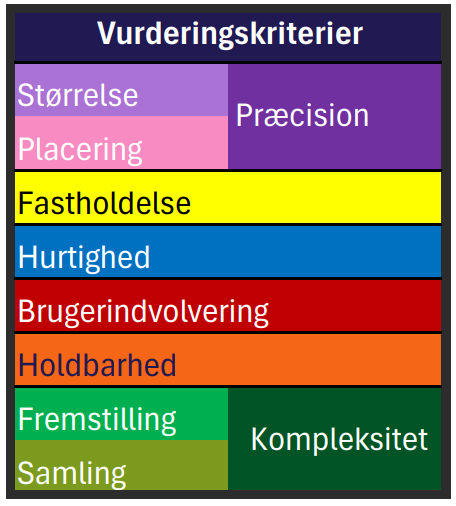
\includegraphics[width=0.25\linewidth]{bilag/Media/Media/delkoncept mekanisk beskrivelse.png}
%\end{figure}

%------
\section{Endelig konceptforslag}

\begin{table}[H]
   \caption{Morfologisk analyse af mekaniske dele. 3 $=$ \protect\cyanbox, 7 $=$ \protect\orangeangle og det endelige koncept sammensat af 3 og 7 kaldet 10 $= \protect\mathcolor{BrickRed}{\clubsuit}$}
    \centering
    \begin{tabular}{|l|p{3.1cm}|p{3.1cm}|p{3.1cm}|p{3.1cm}|} \cline{2-5}      
           \multicolumn{1}{l|}{} & \multicolumn{4}{|c|}{\cellcolor{aaublue} \textcolor{white}{\textbf{Delkoncepter til mekaniske delfunktioner }}} \\ \cline{2-5} \multicolumn{1}{l|}{}  & \multicolumn{1}{c|}{ \cellcolor{lightgray!20} \textbf{1}} & \multicolumn{1}{|c|}{\cellcolor{lightgray!20} \textbf{2}} & \multicolumn{1}{c|}{\cellcolor{lightgray!20} \textbf{3}} & \multicolumn{1}{c|}{\cellcolor{lightgray!20} \textbf{4}}  \\ \cline{2-5} \specialrule{0pt}{0.5pt}{0pt}
          
        %Bevægelse
        \rotatebox[origin=c]{90}{\cellcolor{aaublue} \textcolor{white}{\textbf{Bevægelse }}} & \makecell{Lineær\\ bevægelse  \\ \includegraphics[width=0.98\linewidth]{Sections/5 Konceptgenerering/Media/lineær.png} \\ \orangeangle \ $\protect\mathcolor{BrickRed}{\clubsuit}$ } & \makecell{ Robotarm \\ 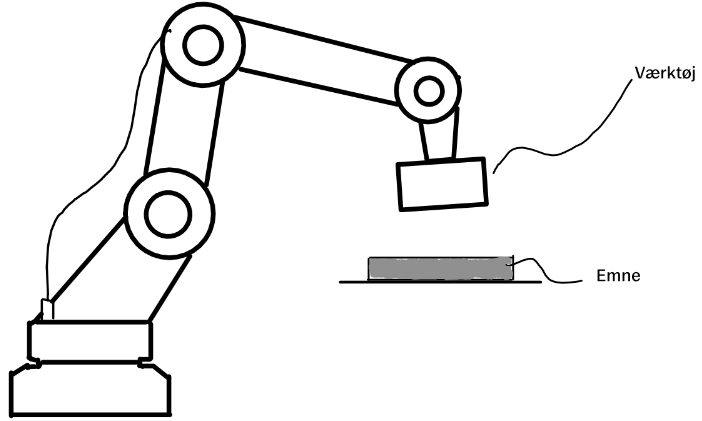
\includegraphics[width=0.98\linewidth]{Sections/5 Konceptgenerering/Media/arm.png} \\} & \makecell{Deltarobot\\ 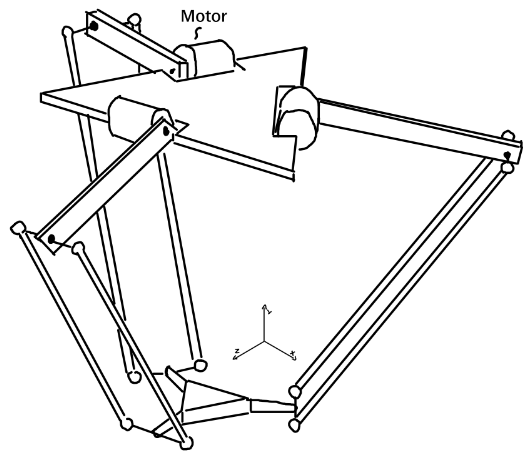
\includegraphics[width=0.98\linewidth]{Sections/5 Konceptgenerering/Media/delta.png} \\ \cyanbox } & \makecell{Drejeskive \\ 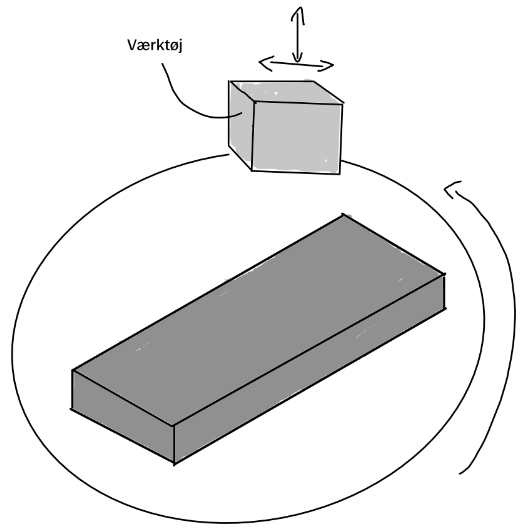
\includegraphics[width=0.98\linewidth]{Sections/5 Konceptgenerering/Media/Drejeskive.png} }\\  \specialrule{1pt}{0pt}{0pt}


        %Sæt prik
        \rotatebox[origin=c]{90}{\cellcolor{aaublue} \textcolor{white}{\textbf{Sætte prikker}}} & \makecell{Sætte dråbe \\ \includegraphics[width=0.98\linewidth]{Sections/5 Konceptgenerering/Media/åbnelukke.png} \\ \cyanbox \ $\protect\mathcolor{BrickRed}{\clubsuit}$} & \makecell{Spids røre  \\ emnet \\ \includegraphics[width=0.3\linewidth]{Sections/5 Konceptgenerering/Media/spids røre.png} \\  \orangeangle } & \makecell{Spray \\ 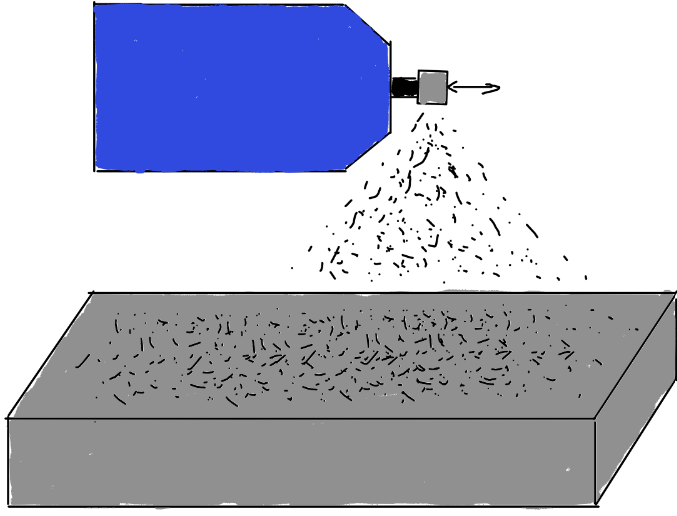
\includegraphics[width=0.98\linewidth]{Sections/5 Konceptgenerering/Media/spray.png}} & \makecell{Stempel \\ 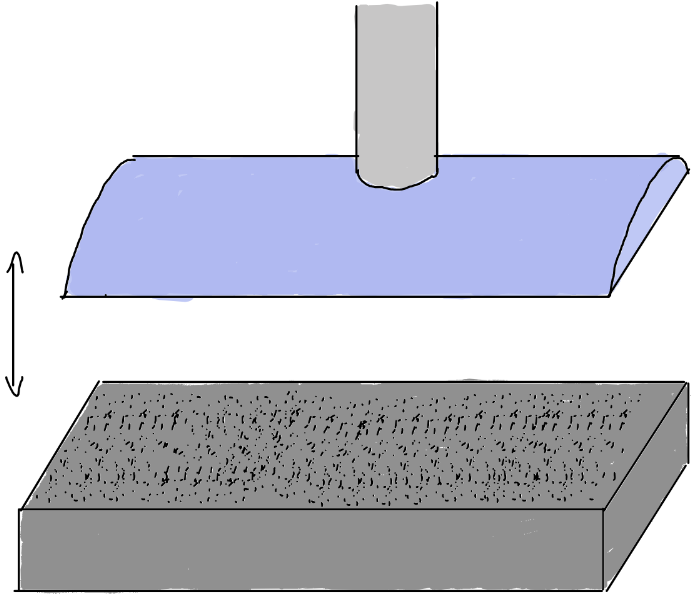
\includegraphics[width=0.98\linewidth]{Sections/5 Konceptgenerering/Media/stempel.png}}  \\ \specialrule{1pt}{0pt}{0pt}

        %Indspænding
        \rotatebox[origin=c]{90}{\cellcolor{aaublue} \textcolor{white}{\textbf{Indspænding}}} & \makecell{Press på \\ emnet \\ \includegraphics[width=0.7\linewidth]{Sections/5 Konceptgenerering/Media/Press på emnet.png} \\ \orangeangle \ $\protect\mathcolor{BrickRed}{\clubsuit}$}  & \makecell{Sug \\ 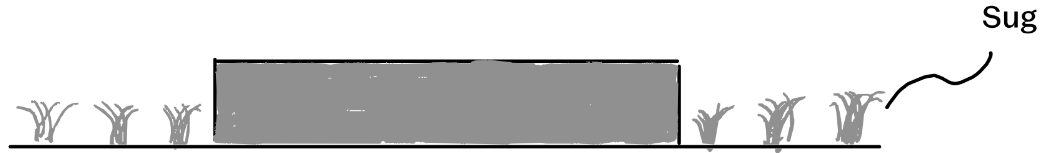
\includegraphics[width=0.98\linewidth]{Sections/5 Konceptgenerering/Media/sug.png} \\ } & \makecell{Vakuumpose\\ med fyld \\ 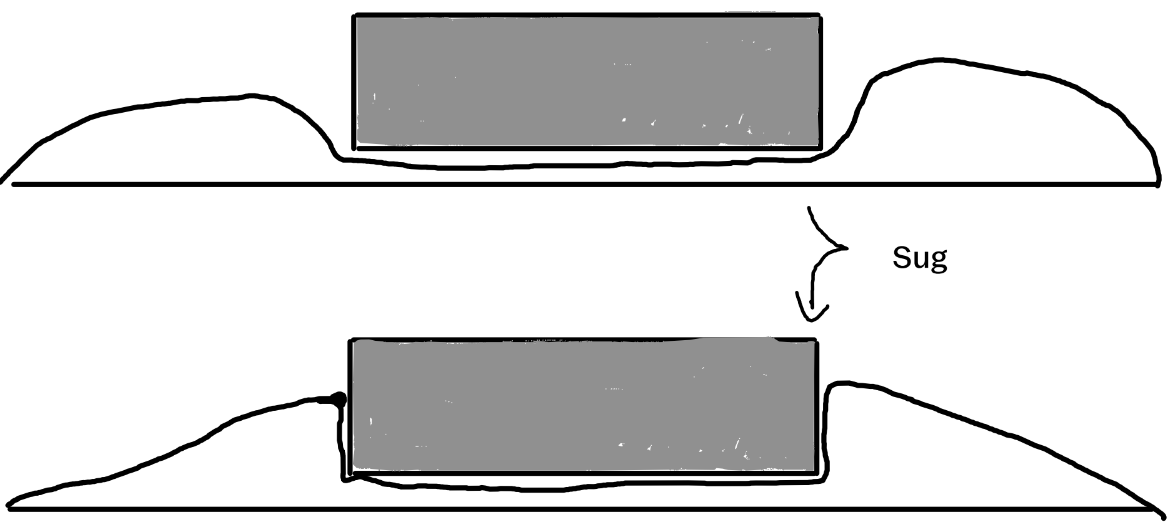
\includegraphics[width=0.98\linewidth]{Sections/5 Konceptgenerering/Media/vakuum.png} \\ \cyanbox }&  \makecell{Ru \\ overflade \\ 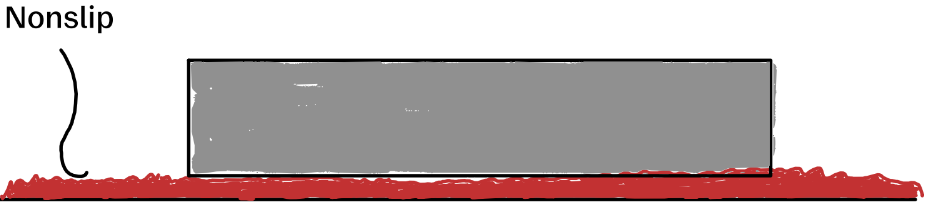
\includegraphics[width=0.98\linewidth]{Sections/5 Konceptgenerering/Media/rug.png} \\}  \\ \specialrule{1pt}{0pt}{0pt}

        %Understøttelse
        \rotatebox[origin=c]{90}{\cellcolor{aaublue} \textcolor{white}{\textbf{Understøttelse}}} & \makecell{Plade \\ under emnet \\ \includegraphics[width=0.98\linewidth]{Sections/5 Konceptgenerering/Media/Understøttelse plade.png} \\ \cyanbox \ \orangeangle  \ $\protect\mathcolor{BrickRed}{\clubsuit}$} & \makecell{Understøttet \\ i punkter \\ \includegraphics[width=0.98\linewidth]{Sections/5 Konceptgenerering/Media/Understøttelse i punkter.png} \\ } & &    \\ \hline
        
    \end{tabular}
\end{table}





\begin{figure}[H]
    \centering
    \includegraphics[width=0.5\linewidth]{Sections/5 Konceptgenerering/Media/10.løsning.png}
    \caption{Skitse af konceptforlag 10 $\protect\mathcolor{BrickRed}{\clubsuit}$}
    \label{fig:Endelig mekaniske koncept}
\end{figure}


\begin{table}[H]
    \centering
    \caption{screening skema for det endelige koncept der er sammensat af koncept 3 \protect\cyanbox \ og 7 \protect\orangeangle, benævnt koncept 10 $\protect\mathcolor{BrickRed}{\clubsuit}$}
    \begin{tabular}{|l|c|| l c l c l c||r|} \cline{2-5}

        \multicolumn{1}{c}{}& \multicolumn{7}{|c|}{\cellcolor{aaublue} \textcolor{white}{\textbf{Konceptforslag til mekaniske dele}}} \\ \hline
         
        \multicolumn{1}{|c}{\cellcolor{lightgray!20}\textbf{Vurderingskriterier}} & \multicolumn{1}{|c||}{\cellcolor{lightgray!20}\textbf{1 \protect\lillacirc}}  & \multicolumn{1}{l}{\cellcolor{lightgray!20} ~} & \multicolumn{1}{c}{\cellcolor{lightgray!20}\textbf{3 \cyanbox}} & \multicolumn{1}{l}{\cellcolor{lightgray!20} ~} & \multicolumn{1}{c}{\cellcolor{lightgray!20}\textbf{7 \orangeangle}} & \multicolumn{1}{l}{\cellcolor{lightgray!20} ~}  &\multicolumn{1}{c||}{\cellcolor{lightgray!20}\textbf{10 $\protect\mathcolor{BrickRed}{\clubsuit}$}} &\multicolumn{1}{r|}{\cellcolor{lightgray!20}\textbf{Vægt}} \\ \hline
         
    %% Vurdering
        % Præcision af prik størrelse
         \multicolumn{1}{|l|}{\cellcolor{aaublue} \textcolor{white}{\textbf{Præcision af prik størrelse}}} 
         & 0 &~& 0&~& -1 &~& 0 & 3\\ \hline
        % Præcision af prik placering  
         \multicolumn{1}{|l|}{\cellcolor{aaublue} \textcolor{white}{\textbf{Præcision af prik placering}}} 
         & 0 && -1 &&  1 &&  0 & 3 \\ \hline
        % Fastholdelse
         \multicolumn{1}{|l|}{\cellcolor{aaublue} \textcolor{white}{\textbf{Fastholdelse}}} 
         & 0 && 1 & &1 && 1 & 5  \\\hline
        % Hurtighed
         \multicolumn{1}{|l|}{\cellcolor{aaublue} \textcolor{white}{\textbf{Hurtighed}}} 
         & 0 && 0 && -1 && 0 & 2 \\\hline
        % Brugerinvolvering
         \multicolumn{1}{|l|}{\cellcolor{aaublue} \textcolor{white}{\textbf{Brugerinvolvering}}} 
         & 0 && 0 && -1 && -1 & 2 \\\hline
        % Holdbarhed
         \multicolumn{1}{|l|}{\cellcolor{aaublue} \textcolor{white}{\textbf{Holdbarhed}}} 
         & 0 && 0 && 0 && 1 & 1 \\\hline
        % Kompleksitet ved fremstilling
         \multicolumn{1}{|l|}{\cellcolor{aaublue} \textcolor{white}{\textbf{Kompleksitet ved fremstilling}}} 
         & 0 && -1 && 2 && 1  & 1 \\\hline
        % Kompleksitet ved samling
        \multicolumn{1}{|l|}{\cellcolor{aaublue} \textcolor{white}{\textbf{Kompleksitet ved samling}}} 
        & 0 && 0 &~& 0 &~& -1 &  1 \\ \hline \specialrule{0pt}{2pt}{0pt} \cline{1-8}
%% Samlet score og rank
         \multicolumn{1}{|r|}{\cellcolor{lightgray!10} \textbf{Vægtet score}}& 0 &~& 1 &~& 3 &~& 4 & \multicolumn{1}{c}{} \\\cline{1-8} 
    \end{tabular}
\end{table}


